\documentclass{article}
\usepackage[utf8]{inputenc}
\usepackage{polski}
\usepackage[polish]{babel}
\usepackage{bbm}
\usepackage{graphicx}    
\usepackage{caption}
\usepackage{subcaption}
\usepackage{epstopdf}
\usepackage{amsmath}
\usepackage{amsthm}
\usepackage{hyperref}
\usepackage{url}
\usepackage{comment}
\newtheorem{defi}{Definicja}
\newtheorem{twr}{Twierdzenie}
\usepackage{listings}
\usepackage{float}


\author{Michał Martusewicz 282023}
\date{Wrocław, \today}
\title{\textbf{Rozważania na temat \textit{Metody Steffensena}}  \\ Sprawozdanie do zadania P.1.17}

\begin{document}
\maketitle
\section{Wstęp}

Wybrane przeze mnie zadanie polega na zaprogramowaniu metody Steffensena dla wybranych funkcji.
Metoda ta służy do znajdowania pierwiastków równania nieliniowego i przy pewnych założeniach jest zbieżna kwadratowo.
 W \S 2 przedstawię ogólnie tą metodę, założenia zbieżności kwadratowej i dowód zbieżności kwadratowej.
 W \S 3 przedstawię kod programu, służącego do obliczania pierwiastków metodą Steffensena.
 W \S 4 porównam metody Newtona i Steffensena na przykładach wybranych funkcji.
 W \S 5 przedłożę problem rozbiegania tej metody.
 W \S 6 rozważę problemy pojawiające się przy funkcjach okresowych.
 W \S 7 podsumuję moje badania.
 
Wszystkie testy numeryczne przeprowadzone są przy użyciu programu \textit{jupyter notebook} i \textit{Julia 0.5.3 (command line version)} w języku \textit{Julia}, używając 
\textit{setprecision(x)} dla x=300.
\section{Wprowadzenie metody}
\textbf{Metodę Steffensena} można przedstawić w następujący sposób:
$$
x_{k+1}:= x_k - f(x_k)/g(x_k),  \qquad k=0,1,...,
$$

gdzie


$$
g(x):=[f(x+f(x))-f(x)]/f(x)
$$

lub


$$
x_{k+1}:=x_k-\frac{f^2(x_k)}{f(x_k+f(x_k))-f(x_k)} \qquad k=0,1,...,
$$
\subsection{Dowód zbieżności kwadratowej metody Steffensena}
Jeżeli przyjmiemy,że $\beta _n =f(x_n)$ i rozwiniemy $g(x_n)$ w szereg Taylora w otoczeniu punktu $x_n$, to otrzymamy 
$$
g(x_n)=\frac{f(x_n+\beta _n)-f(x_n)}{\beta _n}=f'(x_n)\left(1+\frac{1}{2}h_n f''(x_n)+O(\beta _n^2)\right).
$$
gdzie
$$
h_n=\frac{-f(x_n)}{f'(x_n)}
$$
jest poprawką Newtona.Stąd
$$
	x_{n+1}=x_n+h_n\left(1+\frac{1}{2}h_nf''(x_n)+O(\beta_n^2)\right)
$$
Używając wyrażenia ($\epsilon_{n+1}=\frac{1}{2}\epsilon_n^2\frac{f''(\xi}{f'(x_n}$) dla błędu metody Newtona możemy przekształcić tę równość do postaci
$$
h_n=-\epsilon_n+\frac{1}{2}\epsilon_n^2\frac{f''(\xi)}{f'(x_n)}\textrm{, \quad gdzie $\epsilon_n=x_n-\alpha$} 
$$
stąd wynika, że 
$$
\frac{\epsilon_{n+1}}{\epsilon_n^2} \xrightarrow{n\rightarrow\infty} \frac{f''(\alpha)}{2f'(\alpha)}(1+f'(\alpha))
$$
Wynika stąd, że metoda Steffensena zbiega kwadratowo \cite{bib5}.


Warto zauważyć, że $g(x)$ jest przybliżeniem $f'(x)$, więc metoda ta zawsze będzie nieco gorsza niż metoda Newtona. Z drugiej strony metoda Steffensena nie potrzebuje pochodnej, co sprawia że może być użyteczniejsza.

Ze względu na podobieństwo do metody Newtona łatwo zauważyć, że warunkami zbieżności kwadratowej jest brak pierwiastków wielokrotnych w funkcji.
\section{Kod programu}
Zaprogramowanie metody nie jest bardzo skomplikowane, co pokazuje poniższy kod:
\begin{lstlisting}
function steffensen(x0,funkcja,kroki)
    i=0
    while i<kroki
      	last_x=x
        f_x=funkcja(x)
        f2_x=funkcja(x+f_x)
        x=x-(f_x * f_x) / (f2_x-f_x)
        if (isnan(x)||isinf(x))
            x=last_x
            break
        end
        i+=1       
    end
    (x,f_x,-log10(abs(f_x-0.0)))
end
\end{lstlisting}

Funkcja steffensen przyjmuje 3 argumenty. Pierwszym jest punkt początkowy- x0, najlepiej formatu BigFloat. Drugim jest wskaźnik do wybranej funkcji jednoargumentowej, której pierwiastka szukamy. Trzecim jest liczba iteracji. Funkcja ma zaimplementowanego strażnika, który sprawdza czy x nie jest przypadkiem typu NaN (not a number) lub inf ($\infty$). W takim przypadku zwraca ostatnią poprawną wartość x. Funkcja zwraca krotkę, w której znajdują się: wartość znalezionego $x$, wartość $f(x)$ i $-\log_{10}{f(x)}$, co ułatwia tworzenie wykresów.

\section{Porównanie wyników}
Jak już wspomniałem w poprzednim paragrafie dla pewnych wartości metoda Steffensena zbiega kwadratowo, ale zazwyczaj wolniej niż metoda Newtona. Na rysunku \ref{w1a} przedstawiłem wykres dla przykładowej funkcji wielomianowej $f(x)=-5x^5+3x^3+x+3$, która ma jeden pierwiastek w pobliżu $x_0=1.1$ (takie też $x_0$ przyjąłem). Za dokładność metody przyjąłem wartość funkcji w znalezionym przybliżeniu pierwiastka, ze względu na większą dokładność w szacowaniu znalezionego błędu. Na wykresie widać, że zarówno metoda Newtona, jak i metoda Steffensena z każdą iteracją podwajają ilość cyfr dokładnych, choć metoda Newtona nieco szybciej. Obie też przestają rosnąć, gdy dochodzą do granicy dokładności liczby typu BigFloat. Dokładność x 
\begin{figure}[h]
    \centering
    \begin{subfigure}[b]{0.45\textwidth}
        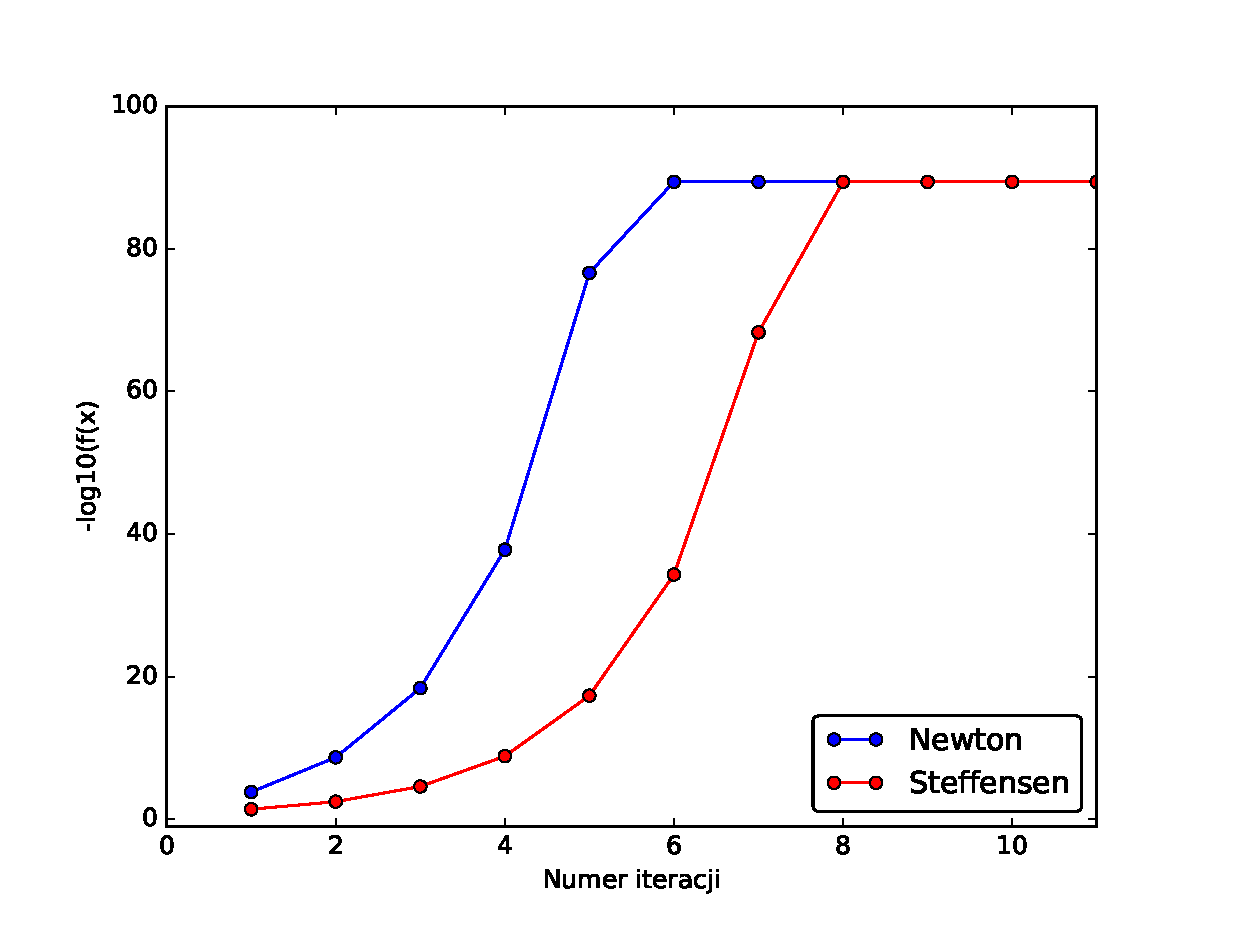
\includegraphics[width=\textwidth]{figure_1.eps}
        \caption{$f(x)=-5x^5+3x^3+x+3$}
        \label{w1a}
    \end{subfigure}
    \begin{subfigure}[b]{0.45\textwidth}
        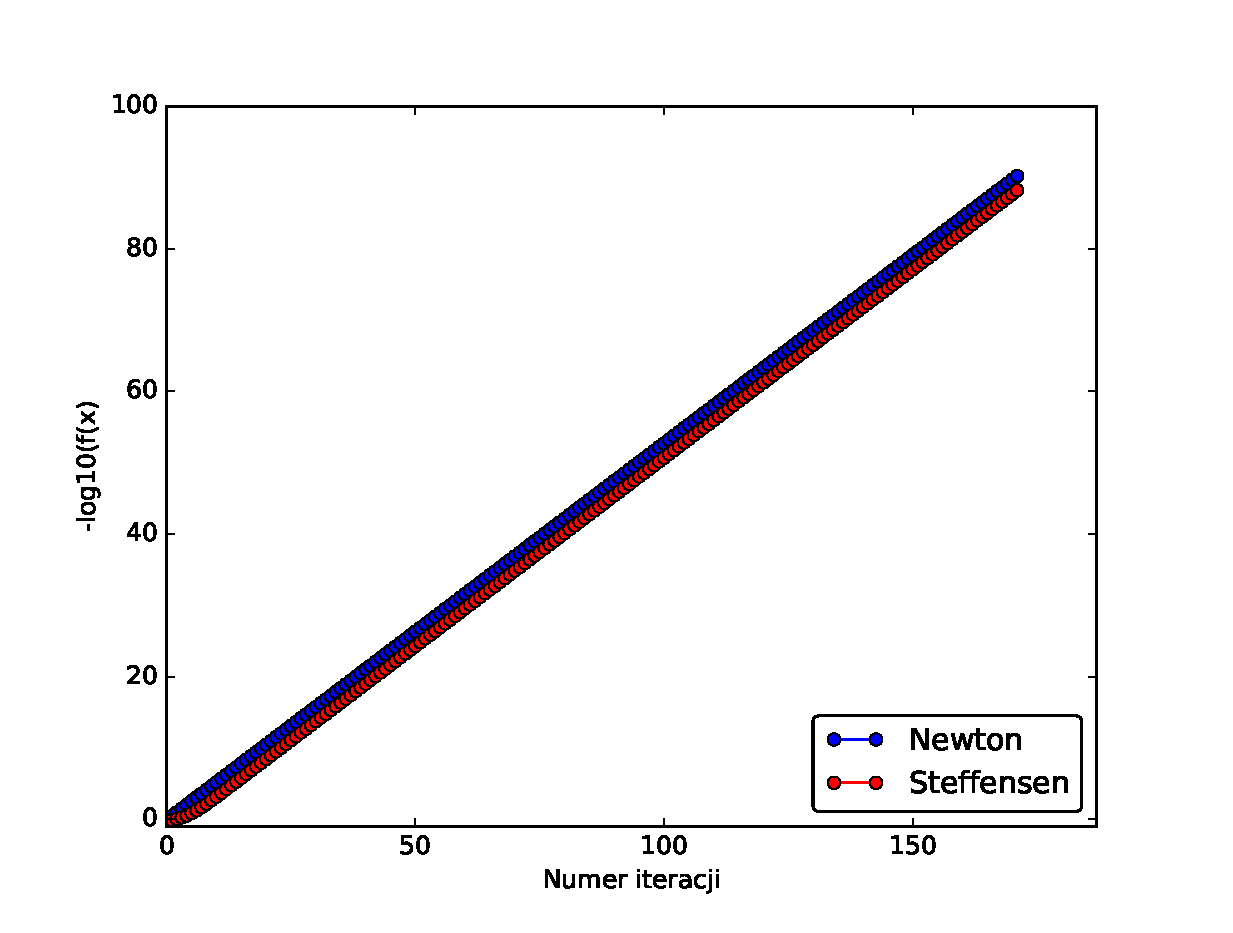
\includegraphics[width=\textwidth]{figure_2.eps}
        \caption{$f(x)=x^3$}
        \label{w1b}
    \end{subfigure}
    \caption{Wykres porównujący liczbę cyfr dokładnych w zależności od iteracji dla metody Newtona i Steffensena dla różnych funkcji}
 	\label{w1}
\end{figure}

Zgodnie z przewidywaniami dla funkcji z pierwiastkami wielokrotnymi obie metody zbiegają liniowo, przy czym metoda Newtona jest nieco szybsza.

\section{Rozbieganie metody}
Jedną z części zadania było wykonanie obliczeń dla funkcji $f(x)=x^3-5x^2+3x -7$. 
Poniżej w tabeli \ref{t1} przedstawiłem kolejne wartości $x$ i $f(x)$ dla tej metody, zaczynając od $x_0=5.0$

\begin{table}[h]
    \centering
    \begin{tabular}{|c|c|c|} 
    \hline
    	$i$ &$x_i$&$f(x_i)$\\\hline
        0 & 5.0 & 8.0 \\
        1 & 4.953488372093023 & 6.719207113839033 \\
        2 & 4.9049667122275595 & 5.428522923637778 \\
        3 & 4.854857045108512 & 4.143604385812245 \\
        4 & 4.804301607434333 & 2.8959287868815795 \\
        5 & 4.755912276218661 & 1.7467894453271677 \\
        6 & 4.7148471377777295 & 8.056550124277053e-1 \\
        7 & 4.688481755866221 & 2.1769447154201013e-1 \\
        8 & 4.67944190876776 & 1.9008599234294415e-2 \\
        9 & 4.678580593806081 & 1.5499478292731384e-4 \\
        10 & 4.678573510902379 & 1.0373026493418519e-8 \\
        11 & 4.678573510428322 & 4.6462848447273136e-17 \\
        12 & 4.678573510428322 & 9.321944665183734e-34 \\
        13 & 4.678573510428322 & 3.7523893936404276e-67 \\
 		\hline
    \end{tabular}
    \caption{Kolejne przybliżenia $f(x)=x^3-5x^2+3x -7$ dla $x_0=5.0$}
	\label{t1}
\end{table}
Postanowiłem głębiej zbadać jak zmienia się zbieżność metody Steffensena w zależności od wybranego $x_0$. Na wykresie \ref{w2} przedstawiłem porównanie zbieżności obu metod. 

Wykresy budowane są w następujący sposób: jeżeli dla danego $x < x_0=5.0$ metoda zbiega do $0$, to zaznaczana jest wartość $1$, jeżeli nie zbiega, to wartość $-1$. dla $x > x_0=5.0$ zaznaczane są analogicznie wartości $3$ i $-3$. Poniżej będą również przykłady dla 2 różnych pierwiastków $x_1$ i $x_2$, wtedy dla $x: x_1<x<x_2$ zaznaczane były wartości odpowiednio $2$ i $-2$. Zielonymi kropkami zaznaczono wybrane pierwiastki.

\begin{figure}[H]
    \centering
	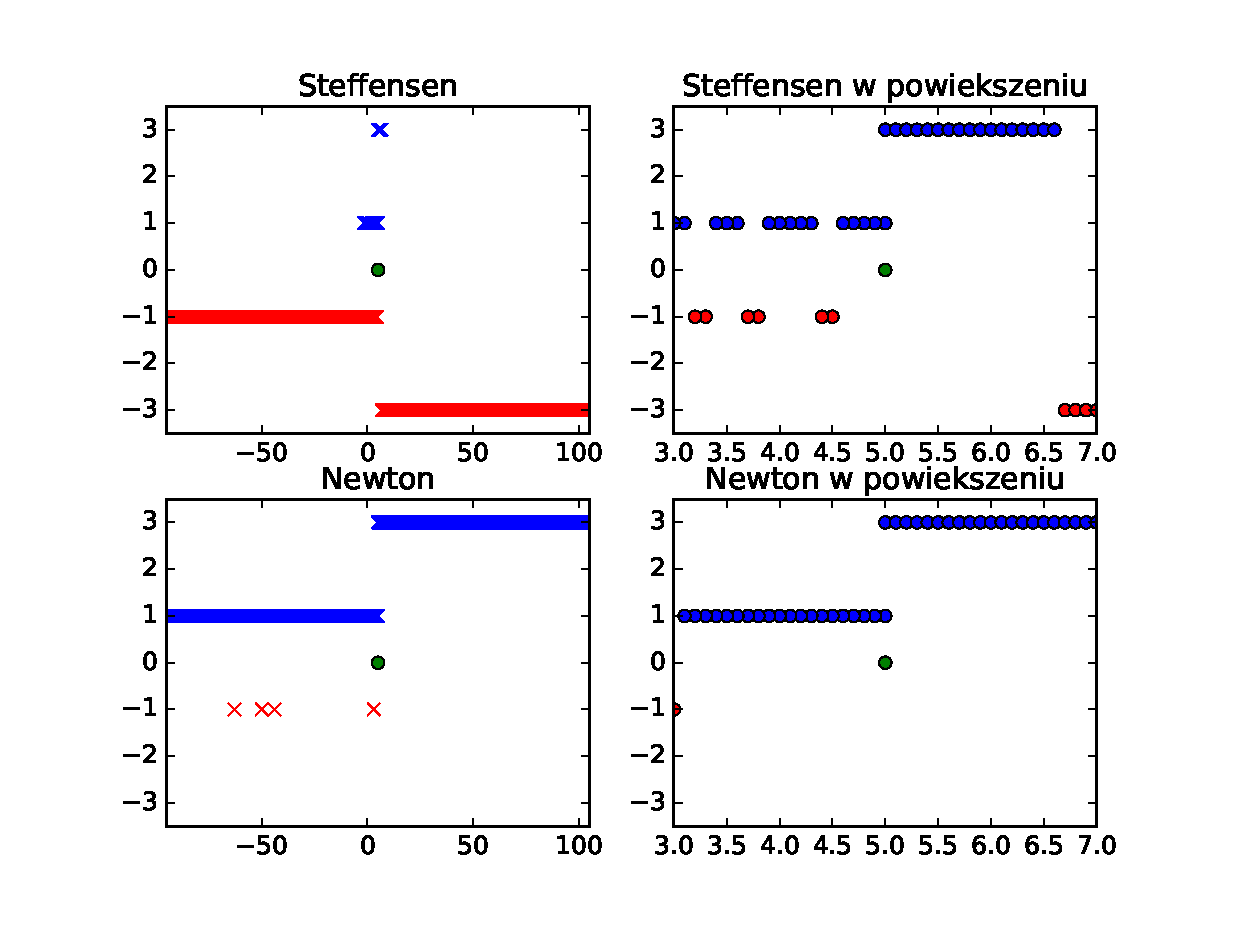
\includegraphics[width= 1 \textwidth]{figure_3.eps}
    \caption{Porównanie rozbiegania metod Newtona i Steffensena w zależności od wyboru punktu początkowego}
 	\label{w2}
\end{figure}
Wykres przedstawia dość interesujące dane. Okazuje się, że metoda Steffensena działa jedynie w ograniczonym zakresie i dla punktów początkowych leżących bardzo blisko rzeczywistego pierwiastka. Jednak jak się okazuje nawet wybór takiego odpowiednio bliskiego punktu nie daje pewności, że otrzymamy poprawny wynik. okazuje się że jest pewien zakres, dla którego wynik jest dość losowy. Dobrze to obrazuje na wykresie nr \ref{w2} część pod tytułem  ,,Steffensen w powiększeniu''. Możemy zobaczyć tam, że dla $x$ z okolic 4.5 metoda rozbiega, ale już dla $x$ z bliskich okolic $3.5$ i 4 zachowuje się poprawnie. Problem ze zbieżnością jest częsty dla metod iteracyjnych, jednak w porównaniu do Metody Newtona, metoda Steffensena zachowuje się dużo mniej stabilnie. Testy dla wielu innych funkcji potwierdzają te obserwacje, jednak ze względu na czytelność sprawozdania nie zamieszczam tu ich wszystkich. Część z nich znajduje się w notatniku IJulia. 

\section{Pierwiastki wielokrotne}
Kolejną częścią zadania było sprawdzenie, jak zachowuje się funkcja $f(x)=x-tg x$ dla $x_0=4.5$ i$x_0=7.7$. Najpierw sprawdziłem szybkość zbieżności dla pierwszego (rysunek \ref{w3a}), a później dla drugiego (rysunek \ref{w3b}). Otrzymane wyniki przedstawiłem odpowiednio w tabeli \ref{t2} i \ref{t3}. O ile pierwszy wykres kształtuje się zgodnie z oczekiwaniami (obie metody zbiegają kwadratowo), to drugi już nie. Poprzednie doświadczenia na funkcjach nieokresowych wykazywały, że stopień zbieżności obu metod jest taki sam.
\begin{figure}[H]
    \centering
    \begin{subfigure}[b]{0.45\textwidth}
        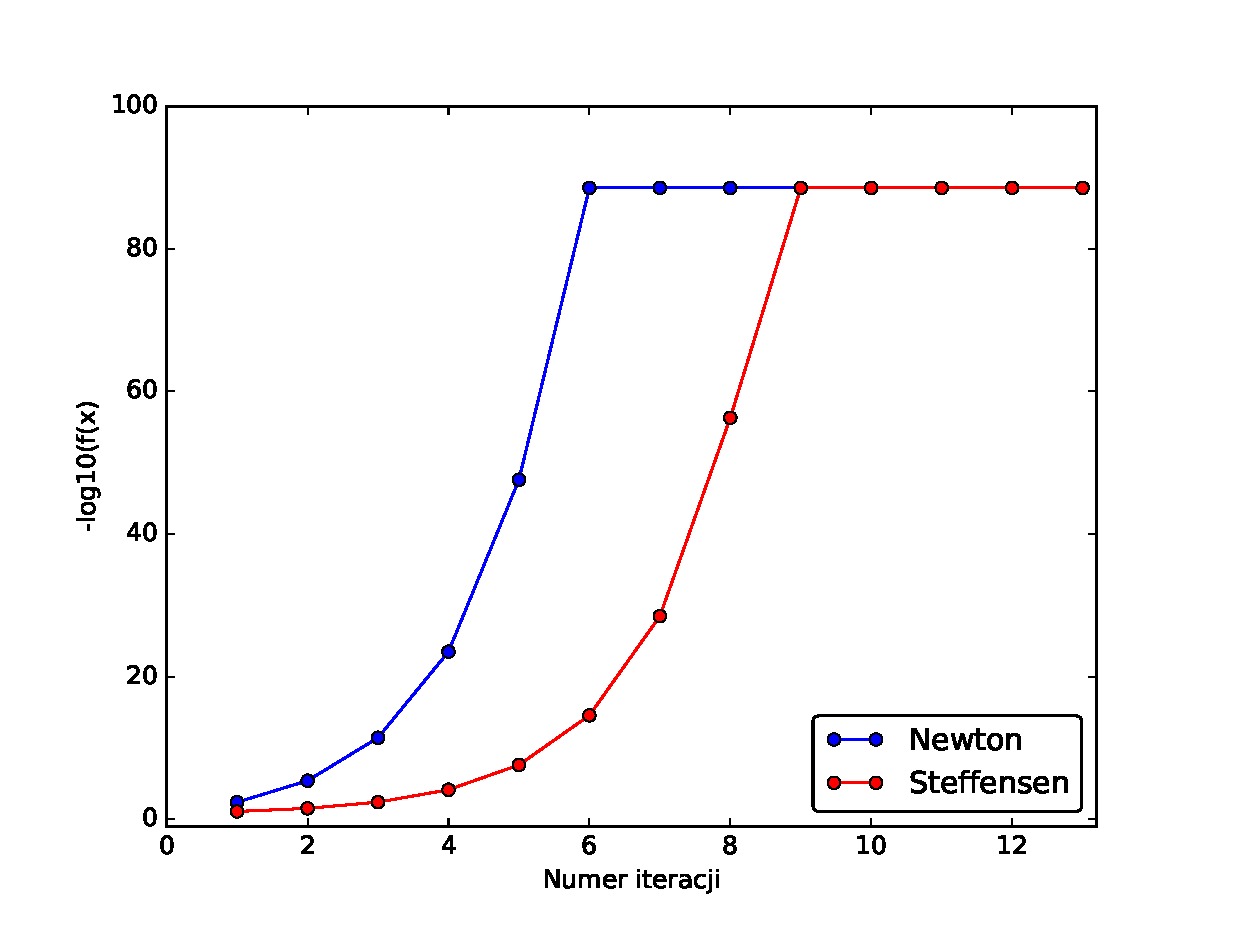
\includegraphics[width=\textwidth]{figure_4a.eps}
        \caption{$x_0=4.5$}
        \label{w3a}
    \end{subfigure}
    \begin{subfigure}[b]{0.45\textwidth}
        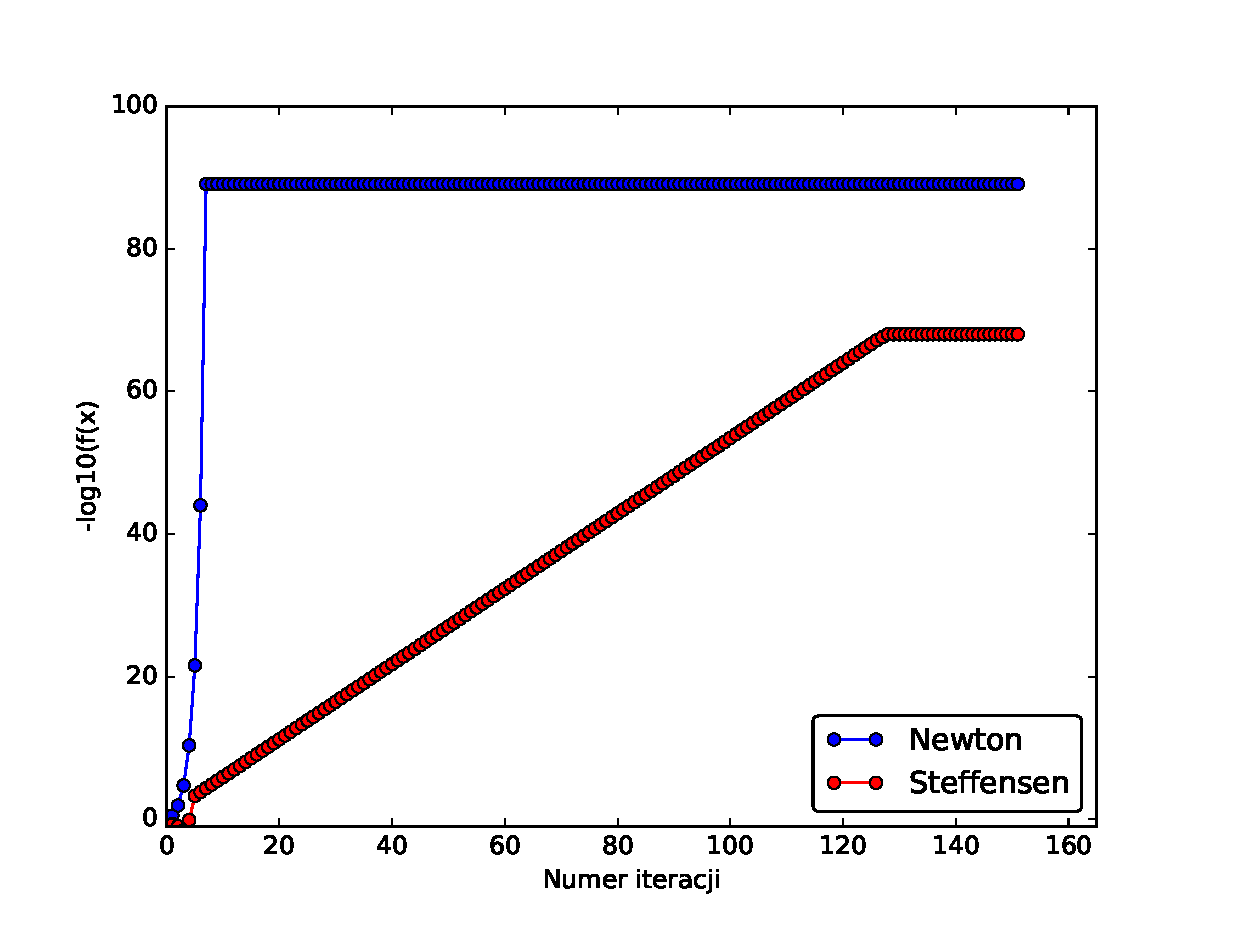
\includegraphics[width=\textwidth]{figure_4b.eps}
        \caption{$x_0=7.7$}
        \label{w3b}
    \end{subfigure}
    \caption{Wykres porównujący liczbę cyfr dokładnych w zależności od iteracji metodą Newtona i Steffensena dla $f(x)=x-tg x$ przy różnych $x_0$}
 	\label{w3}
\end{figure}
\begin{table}[p]
    \centering
    \begin{tabular}{|c|c|c|} 
    \hline
    	$i$ &$x_i$&$f(x_i)$\\\hline
0 & 4.5 & -0.13733205455118447 \\
1 & 4.489272539141293 & 0.08192804446922729 \\
2 & 4.4919085627556665 & 0.03009112943081473 \\
3 & 4.493207908471475 & 0.004065565555118418 \\
4 & 4.493405787163979 & 7.411373462312256e-5 \\
5 & 4.4934094566896325 & 2.4621220821419118e-8 \\
6 & 4.493409457909064 & 2.7172433410635767e-15 \\
7 & 4.493409457909064 & 3.309530836669302e-29 \\
8 & 4.493409457909064 & 4.9095561313914476e-57 \\
9 & 4.493409457909064 & -2.749092340566727e-89 \\
10 & 4.493409457909064 & -2.749092340566727e-89 \\
11 & 4.493409457909064 & -2.749092340566727e-89 \\
12 & 4.493409457909064 & -2.749092340566727e-89 \\
13 & 4.493409457909064 & -2.749092340566727e-89 \\
14 & 4.493409457909064 & -2.749092340566727e-89 \\
 		\hline
    \end{tabular}
    \caption{Kolejne przybliżenia $f(x)=x-\tg x$ dla $x_0=4.5$}
	\label{t2}
\end{table}
\begin{table}[p]
    \centering
    \begin{tabular}{|c|c|c|} 
    \hline
    	$i$ &$x_i$&$f(x_i)$\\\hline
0 & 7.7 & 1.2571275265074489 \\
10 & 0.015311060664995543 & -1.1965622667778609e-6 \\
20 & 0.00026551348029534304 & -6.2393375785786965e-12 \\
30 & 4.604409942128439e-6 & -3.253873719654667e-17 \\
40 & 7.98475127560759e-8 & -1.6969260731242154e-22 \\
50 & 1.3846780311643158e-9 & -8.849630765602556e-28 \\
60 & 2.401243550123219e-11 & -4.615166560751337e-33 \\
70 & 4.164123685966191e-13 & -2.4068532289806853e-38 \\
80 & 7.221227547340986e-15 & -1.2551968362571243e-43 \\
90 & 1.252271335412483e-16 & -6.545970808602792e-49 \\
100 & 2.171630082579523e-18 & -3.41378599669305e-54 \\
110 & 3.765938804317646e-20 & -1.7803218456005513e-59 \\
120 & 6.530712982872287e-22 & -9.284543121763646e-65 \\
130 & 3.042287227193178e-23 & -9.385974879631305e-69 \\
 		\hline
    \end{tabular}
    \caption{Kolejne przybliżenia $f(x)=x-\tg x$ dla $x_0=7.7$}
	\label{t3}
\end{table}



Przeprowadziłem zatem badania mające na celu sprawdzić zbieżność obu metod dla różnych x. Dane zostały przedstawione na rysunkach \ref{w4a} i są nad wyraz interesujące. Okazuje się, że metoda Steffensena jest bardziej stabilna niż Newtona. Co więcej, jest zbieżna na całym badanym obszarze. Ani jedna, ani druga właściwość nie przejawiała się na badanych przeze mnie funkcjach nieokresowych. Wszystko wyjaśniło się na wykresie \ref{w4b}. Przedstawiono na nim wartość znalezionych $x$ takich, że $f(x)=0$. Jak widać na załączonym obrazku metoda Steffensena znajduje tylko jeden pierwiastek ($x=0$)niezależnie od punktu początkowego, zaś metoda Newtona znajduje coraz większe pierwiastki, choć dla niektórych punktów początkowych znalezione wartości są czysto losowe. Badania na innych funkcjach okresowych i mieszano-okresowych wykazują, że generalnie metoda Steffensena dla przeważającej większości punktów początkowych znajduje pierwiastek w $x_0=0$, dla niektórych przypadków też inne pierwiastki.

\begin{figure}[H]
    \centering
    \begin{subfigure}[H]{0.9\textwidth}
        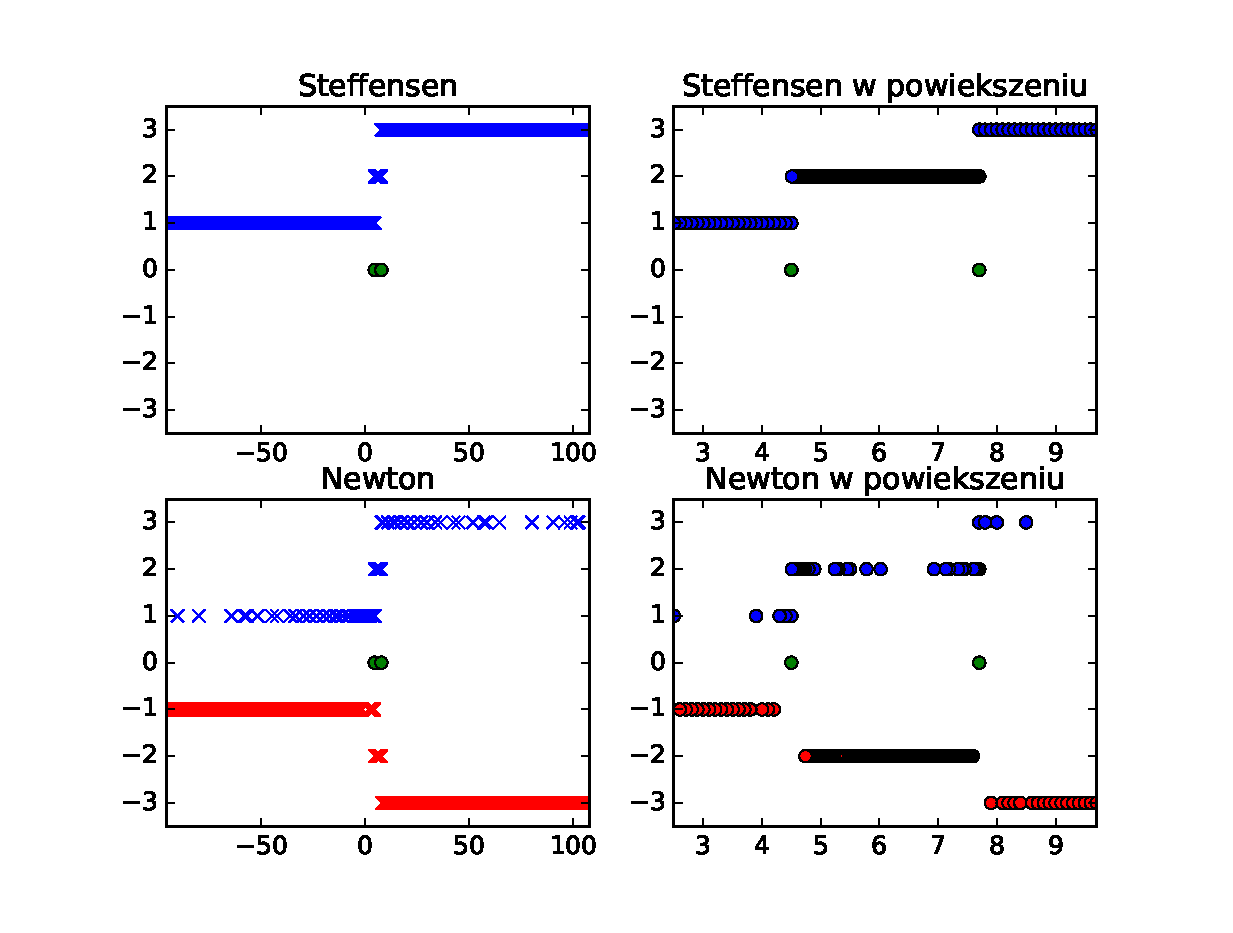
\includegraphics[width=\textwidth]{figure_5.eps}
        \caption{Wykres pokazujący zbieżność metod w zależności od wyboru $x_0$.}
        \label{w4a}
    \end{subfigure}
    \begin{subfigure}[H]{0.9\textwidth}
        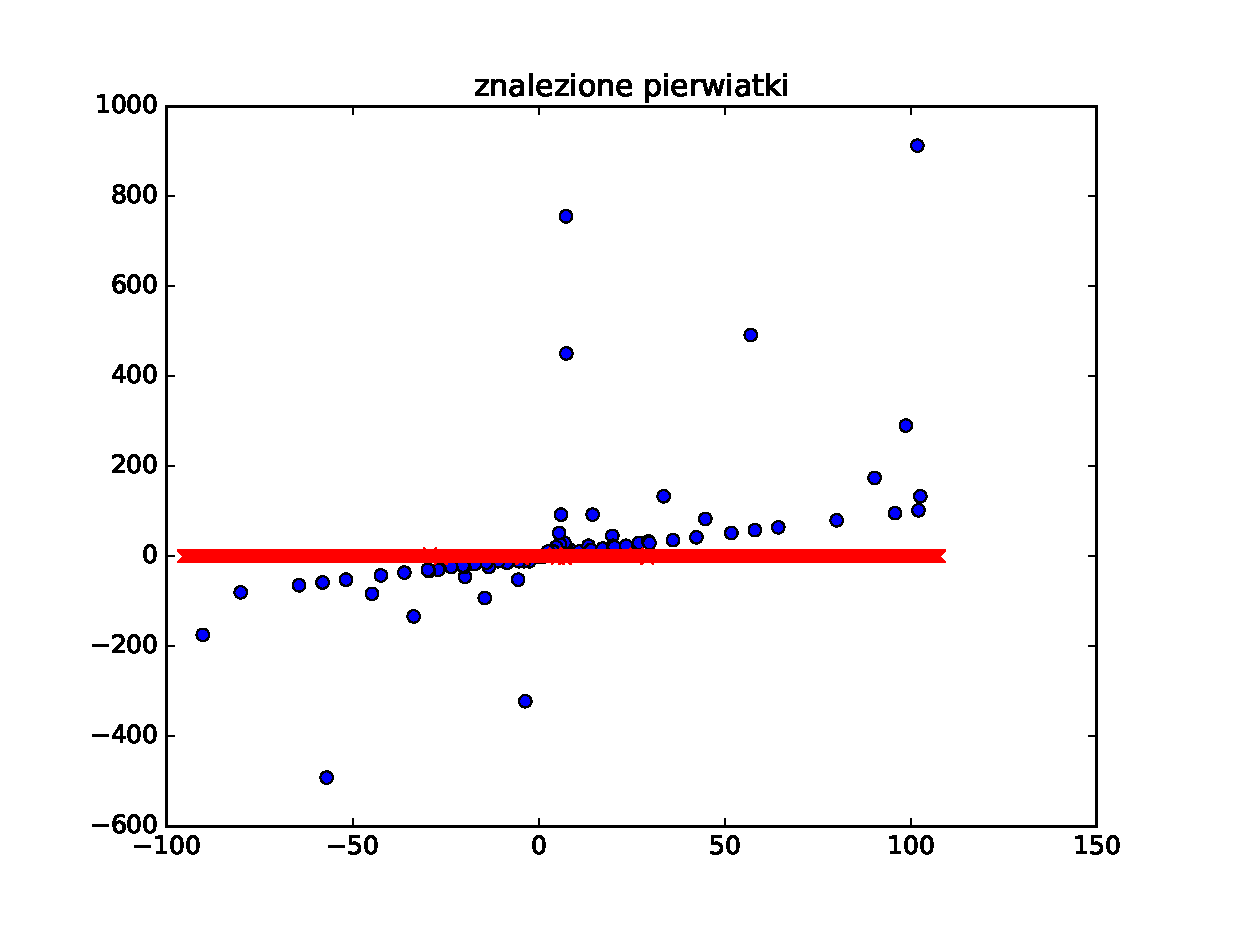
\includegraphics[width=\textwidth]{figure_6.eps}
        \caption{Wykres znalezionych pierwiastków w zależności od wyboru punktu początkowego.}
        \label{w4b}
    \end{subfigure}
    \caption{Wykres obrazujący zachowanie się metod dla $f(x)=x-tg x$ przy różnych $x_0$.}
 	\label{w4}
\end{figure}


\section{Wnioski}
Główną przewagą metody Steffensena nad metodą Newtona jest brak potrzeby podania pochodnej funkcji której pierwiastków szukamy. Jest to wygodne, bo dla większości funkcji jedyną możliwością znalezienia dokładnej funkcji jest rozwiązanie symboliczne, albo przybliżenie.
Kolejną zaletą jest (w przeciwieństwie do metody siecznych) jest zbieżność kwadratowa.

Metoda ta nie jest jednak zbyt powszechnie używana ze względu na swoje liczne wady. Największą jest olbrzymia niestabilność, nawet rozpoczęcie bardzo blisko pierwiastka może rozbiegać, albo wskazywać zupełnie inny pierwiastek. Kolejną wadą jest potrzeba podania bardzo dokładnego punktu początkowego, gdyż jak pokazują doświadczenia, w niektórych przypadkach tylko niewielki zbiór dookoła właściwego pierwiastka zbiega do niego. Dodatkową wadą jest przybliżanie pochodnej, co siłą rzeczy zwiększa niedokładność.

Wszystko to powoduje, że przy braku informacji o pochodnej funkcji użyteczniejsza jest bisekcja, choć warto się zastanowić nad połączeniem tych dwóch metod w złożonych algorytmach znajdujących pierwiastki równań nieliniowych.


\begin{thebibliography}{9}
	\itemsep2pt
	\bibitem{bib1} \url{http://home.agh.edu.pl/~dziembaj/Old/skrypt%20end/podstrony/steffensen.html}
	(ostatni dostęp do strony \today)
	
	\bibitem{bib2} \url{https://en.wikipedia.org/wiki/Steffensen's_method}
	(ostatni dostęp do strony \today)
    \bibitem{bib3} David Kincaid, Ward Cheney. Analiza numeryczna 

   \bibitem{bib5} A. Bjorck G. Dahlquist - Metody numeryczne (przekład S. Paszkowski, wydanie drugie, Warszawa 1987)
    
		
\end{thebibliography}

\end{document}

\section{Wnioski}




\begin{thebibliography}{9}
	\itemsep2pt
	\bibitem{bib1} \url{http://home.agh.edu.pl/~dziembaj/Old/skrypt%20end/podstrony/steffensen.html}
	(ostatni dostęp do strony \today)
	
	\bibitem{bib2} \url{https://en.wikipedia.org/wiki/Steffensen's_method}
	(ostatni dostęp do strony \today)
    \bibitem{bib3} David Kincaid, Ward Cheney. Analiza numeryczna 
    \bibitem{bib3} \url{http://bit.ly/2fgKejw}
	(ostatni dostęp do strony \today)
   \bibitem{bib5} A. Bjorck G. Dahlquist - Metody numeryczne (strona 225)
    
		
\end{thebibliography}

\end{document}